\chapter{几何像差}

\begin{introduction}
	\item 球差(第 \ref{subsect:spherical-aberration} 节)
	\item 彗差(第 \ref{subsect:coma} 节)
	\item 像散(第 \ref{subsect:astigmatism} 节)
	\item 场曲(第 \ref{subsect:field-curvature} 节)
	\item 畸变(第 \ref{subsect:distortion} 节)
	\item 色差(第 \ref{sect:chromatic-aberration} 节)
\end{introduction}

像差是光学系统成像不完善程度的描述。像差可分为单色像差和色差。单色像差包括轴上像差——球差,以及轴外像差——彗差、像散、场曲、畸变。色差可分为位置色差和倍率色差。
\section{轴上像差}
\subsection{球差}
\label{subsect:spherical-aberration}
\begin{definition}{球差}{spherical-aberration}
在第 \ref{subsect:paraxial-ray} 章节中已知,由光轴上一点发出的光线经球面折射后所得的截距$L'$,随入射光线与光轴的夹角$U$或入射光线在球面上的入射点高度$h$而异。轴上点发出的同心光束经光学系统各个球面折射后,将不复为同心光束(如\figref{fig:spherical-aberration-1} 所示)。不同倾角的光线交光轴于不同位置上,相对于理想像点的位置有不同的偏离。这是单色光的成像缺陷之一,称为球差。
\end{definition}

\begin{figure}[htbp]
	\centering
	\begin{minipage}[t]{0.3\textwidth}
		\centering
		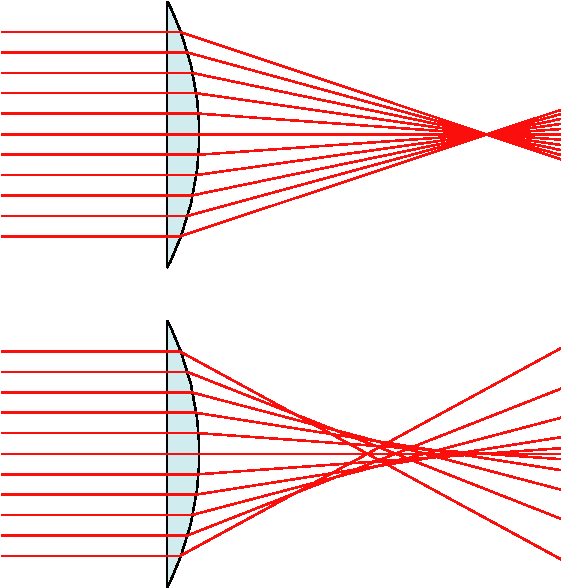
\includegraphics[width=1\textwidth]{spherical-aberration-1.pdf}
		\caption{球差示意图}
		\label{fig:spherical-aberration-1}
	\end{minipage}
	\quad
	\begin{minipage}[t]{0.65\textwidth}
		\centering
		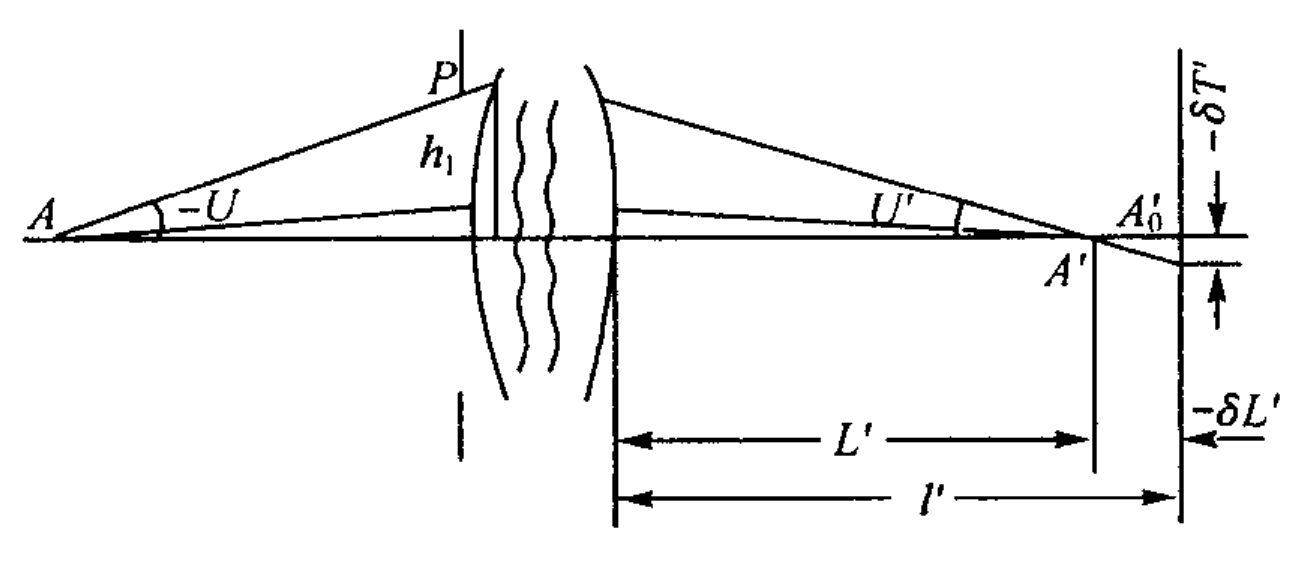
\includegraphics[width=1\textwidth]{spherical-aberration-2.png}
		\caption{球差详解图}
		\label{fig:spherical-aberration-2}
	\end{minipage}
\end{figure}

在\figref{fig:spherical-aberration-2} 中,轴上点$A$的理想像为$A'_0$,由$A$点发出的过入瞳边缘的光线$AP$(边缘光线)从系统出射后,交光轴于$A'$。由于球差,$A'$与$A'_0$不重合。若它们的像方截距分别为$L'$和$l'$,则
\begin{equation}
\delta L'=L'-l'
\label{eq:spherical-aberration}
\end{equation}
为\textbf{轴向球差}。\figref{fig:spherical-aberration-2} 所示的是$\delta L'<0$的情况。若使某一孔径带$\delta L'=0$,称光学系统对这一环带光线校正球差。大部分光学系统只能对一环带光线校正球差,一半是对边缘光线校正。这种光学系统叫做\textbf{消球差系统}。

球差对成像质量的危害,是它在理想像平面上引起半径为$\delta T'$的弥散圆。$\delta T'$为\textbf{垂轴球差},它与轴向球差$\delta L'$之间有如下关系:
\begin{equation}
\delta T'=\delta L'\cdot\tan U'
\label{eq:spherical-aberration-relationship}
\end{equation}

轴上点以单色光成像时只有球差,但轴上点以近轴细光束所成的像是理想的。由此可见,轴上点球差完全是由于光束的孔径角增大而引起的。所以,大孔径系统只允许有足够小的球差。同时可以看出,球差必然是$U_1$或$h_1$的函数。可以简单地把球差表示成$U_1$或$h_1$的幂级数。考虑到当$U_1$或$h_1$变号时球差不变,当$U_1$或$h_1$为零时球差为零,可以得出
\begin{equation}
\begin{cases}
\delta L'=A_1h^2_1+A_2h^4_1+A_3h^6_1+\cdots\\
\delta L'=a_1u^2_1+a_2u^4_1+a_3u^6_1+\cdots
\end{cases}
\end{equation}
结合式(\ref{eq:spherical-aberration-relationship})可得垂轴像差为
\begin{equation}
\begin{cases}
\delta T'=B_1h^2_1+B_2h^4_1+B_3h^6_1+\cdots\\
\delta T'=b_1u^2_1+b_2u^4_1+b_3u^6_1+\cdots
\end{cases}
\end{equation}
展开式中第一项为\textbf{初级球差},此后各项分别为二级球差、三级球差等,二级以上的球差统称为\textbf{高级球差}。大部分光学系统二级以上的球差很小,可以忽略。
\begin{property}
	初级球差与孔径的平方成正比,二级球差与孔径的$4$次方成正比。当孔径较小时,主要存在初级球差;当孔径较大时,高级球差增大。	
\end{property}

球差的精确数值须对光线作光路计算后按照式(\ref{eq:spherical-aberration})求得。但对于仅有初级球差的系统,只需要计算一条光线,通常是边缘光线的球差,即可求得公式中的系数$A_1$或$a_1$,从而求知其他带的球差。同理,若同时有初级和二级球差,只要计算两条光线的求差值,即可确定各项系数,并求得其他各带的球差。大多数光学系统属于此类,对于这种系统,利用初级球差和二级球差的平衡,可以对一个孔径带校正球差,此时在其他带上必定具有\textbf{剩余球差}。

以光线的相对高度表示展开式
\begin{equation}
\delta L'=A_1\bigg(\frac{h_1}{h_m}\bigg)^2+A_2\bigg(\frac{h_1}{h_m}\bigg)^4
\end{equation}
当对$h=h_m$的边光消球差时,有$A_1=-A_2$,为求得球差的极值,将上式对$h$微分,并令其为零,得
\begin{equation}
h_1=\frac{1}{\sqrt{2}}h_m=0.707h_m
\end{equation}
即当边光球差为零时,$h_1=0.707h_m$这一带光线,通常称带光,具有最大的剩余球差,其值为
\begin{equation}
\delta L'_{\max}=0.25A_1=-0.25A_2
\end{equation}
\begin{conclusion}
对于可用展开式中前两项来描述球差的光学系统,当对边光校正了球差后,在$0.707$高度的带光具有最大的剩余球差。其值是边光为平衡高级球差所需的初级球差的$1/4$。若高级球差为正,带球差一定为负。光学系统的高级球差越大,带球差也越大;反之,已对边光消球差的系统,带球差大者,高级球差必大。
\end{conclusion}
\begin{note}
	\begin{enumerate}
		\item $h_1(u_1)$很小很小,$\delta L'=0$,近轴区。
		\item $h_1(u_1)$很小,仅有初级量,赛得区。只需要确定一条边光确定系数$A_1(a_1)$。
		\item $h_1(u_1)$有一定大小,$4$次项不可略,此时,需要按照上文分析得到最大剩余球差$\delta L'_{\mathrm{max}}=0.25A_1=-0.25A_2$。
		\item $h_1(u_1)$大时,比如到三级,则须计算三条光线(边光、$0.707$带光、$0.85$带光),校正后,$0.85$带光有最大剩余球差。
	\end{enumerate}
\end{note}

\subsection{球差曲线}
以$\delta L'$为横坐标,$h/h_m$为纵坐标,可以画出如\figref{fig:spherical-aberration-curve-1} 所示的球差曲线,它能明晰地反映出系统的球差性质和球差校正情况。以$(h/h_m)^2$为纵坐标绘制的球差曲线如\figref{fig:spherical-aberration-curve-1} 所示,该图与波像差联系密切,且易于反映系统的球差性质。如果仅有初级球差,将得到一条直线;若不为直线,则在曲线上纵坐标为零处作的切线与曲线的偏离即为系统的高级球差。

\begin{figure}[htbp]
	\centering
	\begin{minipage}[t]{0.45\textwidth}
		\centering
		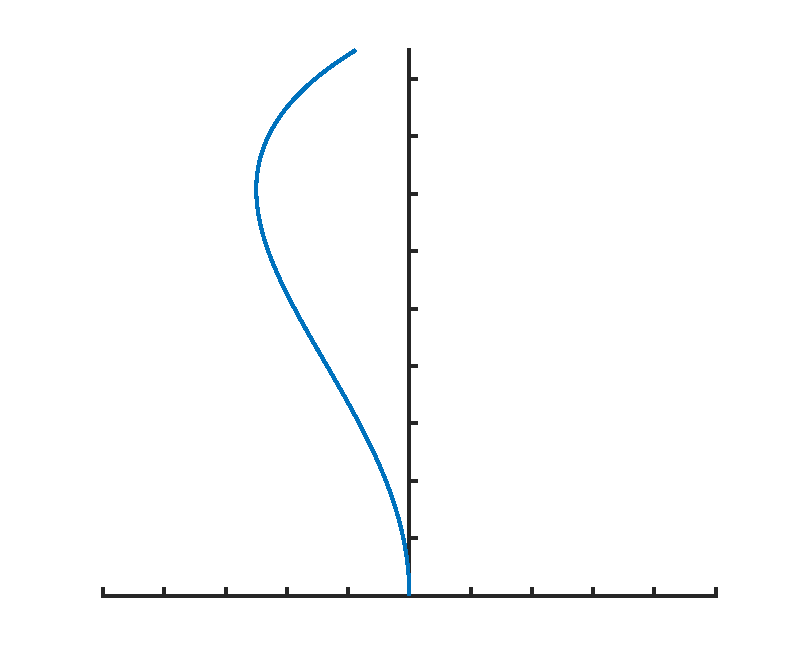
\includegraphics[width=0.8\textwidth]{spherical-aberration-curve-1.pdf}
		\caption{球差曲线($\delta L'\sim h/h_m$)}
		\label{fig:spherical-aberration-curve-1}
	\end{minipage}
	\ 
	\begin{minipage}[t]{0.45\textwidth}
		\centering
		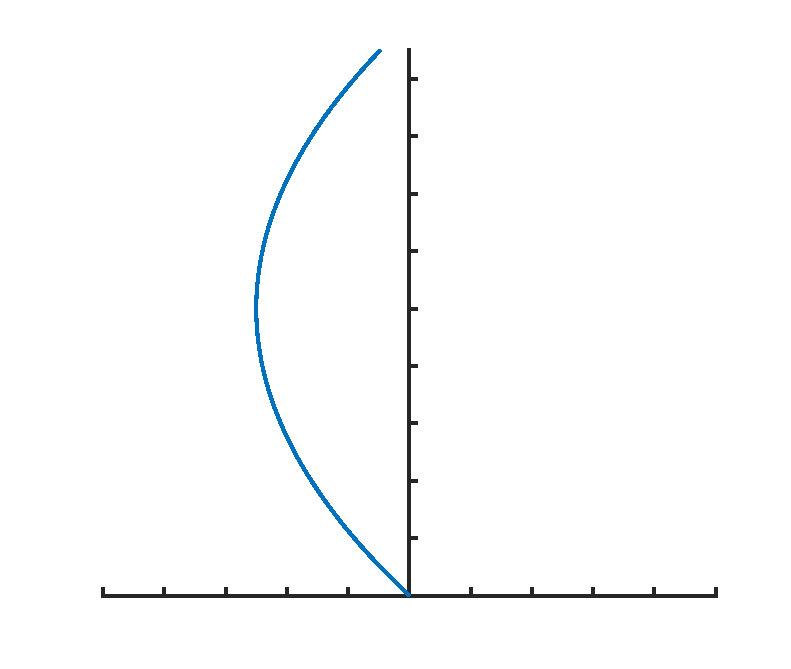
\includegraphics[width=0.8\textwidth]{spherical-aberration-curve-2.pdf}
		\caption{球差曲线($\delta L'\sim (h/h_m)^2$)}
		\label{fig:spherical-aberration-curve-2}
	\end{minipage}
\end{figure}

\subsection{单折射球面的球差}
\label{subsect:aplanatic-point}

假设某一面的物方已有球差,如\figref{fig:spherical-aberration-of-the-object} 所示,经推导可得
\begin{equation}
n'u'\sin U'\delta L'-nu\sin U\delta L=-(L'\sin U'-L\sin U)ni
\label{eq:single-spherical-aberration}
\end{equation}
令$S_{-}=2(L'\sin U'-L\sin U)ni$,则
\begin{equation}
\delta L'=\frac{nu\sin U}{n'u'\sin U'}\delta L-\frac{1}{2n'u'\sin U'}S_{-}
\end{equation}
可见,某表面像空间的球差由两部分构成,即物方球差在像空间的贡献和表面本身所产生的球差。前者通过相当于轴向放大率的因子$(nu\sin U)/(n'u'\sin U')$反映到像空间,后者由$S_{-}$决定。$S_{-}$称为表面的球差分布系数,表征该表面对最后球差的贡献量。利用公式
\begin{equation}
\frac{L'\sin U'}{\cos\bigg(\dfrac{I'-U'}{2}\bigg)}=\frac{L\sin U}{\cos\bigg(\dfrac{I-U}{2}\bigg)}
\end{equation}
$S_{-}$可化为
\begin{equation}
S_{-}=\frac{niL\sin U(\sin I'-\sin U)(\sin I-\sin I')}{\cos{\dfrac{I-U}{2}}\cos{\dfrac{I'+U}{2}}\cos{\dfrac{I+I'}{2}}}
\label{eq:spherical-aberration-distribution-coefficient}
\end{equation}
该式为表征球面产生球差的重要表达式。可见,单个球面在三种情况下不产生球差:
\begin{enumerate}
	\item $L=0$,此时$L'=0$,即不论$U$角多大,射向顶点的光线都从顶点折射而出,不产生球差。
	\item $\sin I-\sin I'=0$,此时$I=I'=0$,即$L=r$,物点位于球心。此时物点发出的所有光线均无折射地通过球面,像点仍在球心,即$L'=r$。
	\item $\sin I'-\sin U=0$或$I'=U$,易求出对应的物像点位置分别为
	\begin{equation}
	L=\frac{n+n'}{n}r,\quad L'=\frac{n+n'}{n'}r
	\end{equation}
	由此可见,这一对无球差的共轭点位于球心的一侧,且都在球心之外,只能是实物成虚像或虚物成实像。物像之间的关系满足
	\begin{equation}
	\frac{\sin U'}{\sin U}=\frac{\sin I}{\sin I'}=\frac{n'}{n}=\frac{L}{L'}
	\label{eq:aplanatic-point}
	\end{equation}
\end{enumerate}

\begin{figure}[htbp]
	\centering
	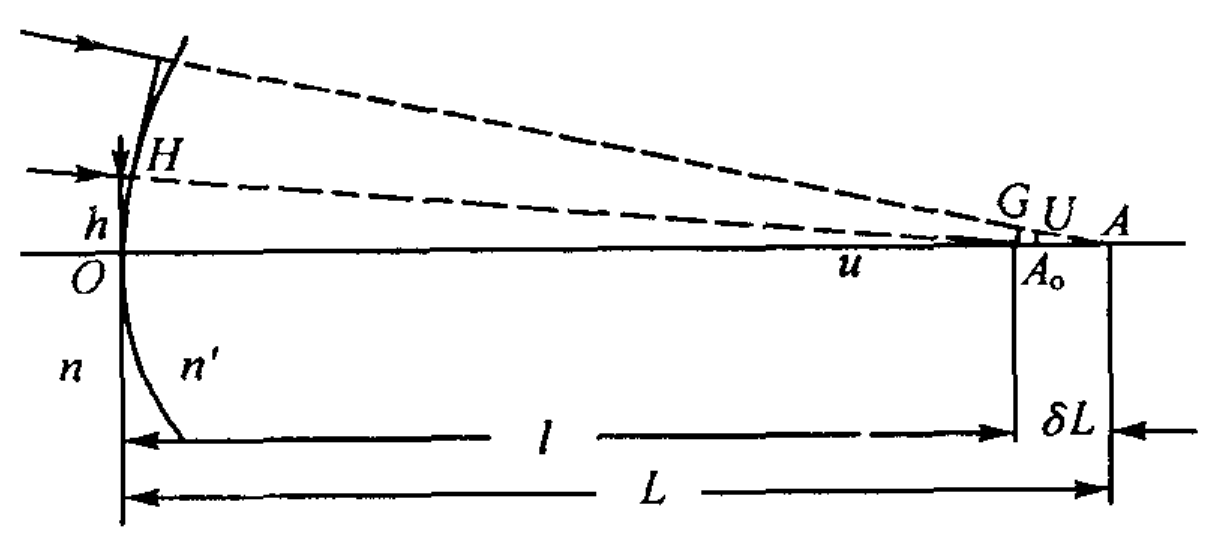
\includegraphics[width=0.6\textwidth]{spherical-aberration-of-the-object.png}
	\caption{物方的球差}
	\label{fig:spherical-aberration-of-the-object}
\end{figure}

\begin{definition}{齐明点}{aplanatic-point}
	由式(\ref{eq:aplanatic-point})可知,不论孔径角多大,这对共轭点的$\sin U'/\sin U$和$L/L'$均为常数,都不产生球差。这一对共轭点能以任意宽的光束对轴上点成完善像,且过该点的垂轴平面上与之很靠近的点也能以任意宽的光束成完善像。故称这对共轭点为齐明点。
\end{definition}

根据单个折射球面的三个无球差的物点位置,可将整个物空间分成四个以这三个点为界的区域。由公式(\ref{eq:spherical-aberration-distribution-coefficient})可知,球差的正负是由$L\sin U$、$i$、$\sin I-\sin I'$和$\sin I'-\sin U$这四个因子的正负决定的:
\begin{enumerate}
	\item 第一因子$L\sin U=PA\cdot[\cos(I-U)/2]$总与$PA$\footnote{$PA$是顶点到光线与球面交点的距离,以顶点为基准上正下负。}同号。
	\item 第二因子$i$与$\sin I$同号。
	\item 第三因子$\sin I-\sin I'=\sin I\cdot(n'-n)/n'$,其正负根据$n$和$n'$的相对大小易于确定。
	\item 第四因子$\sin I'-\sin U$可表示为$n\sin U\cdot[L/r-(n'+n)n]/n'$,其正负随不同区域而异。
\end{enumerate}
在$PA>0$的情况下分别对$r>0$和$r<0$的上述各因子进行正负判断分别得到如\tabref{tab:spherical-aberration-of-sphere-in-each-interval-1} 和\tabref{tab:spherical-aberration-of-sphere-in-each-interval-2} 所示结果。

\begin{table}[htbp]
	\centering
	\caption{$r>0$的球面在各区间内的球差正负}
	\resizebox{\textwidth}{!}{
	\begin{tabular}{c|c|c|c|c|c|c|c|c}
		\hline
		\multirow{2}{*}{} & \multicolumn{2}{c|}{$-\infty\leqslant L<0$} & \multicolumn{2}{c|}{$0<L<r$} & \multicolumn{2}{c|}{$r<L<(n'+n)r/n$} & \multicolumn{2}{c}{$(n'+n)r/n<L\leqslant\infty$}\\
		\cline{2-9} 
		& $n'>n$ & $n'<n$ & $n'>n$ & $n'<n$ & $n'>n$ & $n'<n$ & $n'>n$ & $n'<n$\\
		\hline
		$L\sin U+$& $+$ & $+$ & $+$ & $+$ & $+$ & $+$ & $+$ & $+$\\
		\hline
		$i$或$\sin I+$& $+$ & $-$ & $-$ & $+$ & $+$ & $+$ & $+$ & $+$\\
		\hline
		$\sin I-\sin I'$& $+$会聚 & $-$发散 & $-$发散 & $+$会聚 & $+$会聚 & $-$发散 & $+$会聚 & $-$发散\\
		\hline
		$\sin I'-\sin U$& $+$ & $+$ & $-$ & $-$ & $-$ & $-$ & $+$ & $+$\\
		\hline
		$S\_$& $+$ & $-$ & $-$ & $+$ & $-$ & $+$ & $+$ & $-$\\
		\hline
		$\delta L'$& $-$ & $+$ & $+$ & $-$ & $+$ & $-$ & $-$ & $+$\\
		\hline
	\end{tabular}}
	\label{tab:spherical-aberration-of-sphere-in-each-interval-1}
\end{table}

\begin{table}[htbp]
	\centering
	\caption{$r<0$的球面在各区间内的球差正负}
	\resizebox{\textwidth}{!}{
	\begin{tabular}{c|c|c|c|c|c|c|c|c}
		\hline
		\multirow{2}{*}{} & \multicolumn{2}{c|}{$-\infty\leqslant L<(n'+n)r/n$} & \multicolumn{2}{c|}{$(n'+n)r/n<L<r$} & \multicolumn{2}{c|}{$r<L<0$} & \multicolumn{2}{c}{$0<L\leqslant\infty$}\\
		\cline{2-9} 
		& $n'>n$ & $n'<n$ & $n'>n$ & $n'<n$ & $n'>n$ & $n'<n$ & $n'>n$ & $n'<n$\\
		\hline
		$\sin I-\sin I'$& $-$发散 & $+$会聚 & $-$发散 & $+$会聚 & $+$会聚 & $-$发散 & $-$发散 & $+$会聚\\
		\hline
		$\delta L'$& $+$ & $-$ & $-$ & $+$ & $-$ & $+$ & $+$ & $-$\\
		\hline
	\end{tabular}}
	\label{tab:spherical-aberration-of-sphere-in-each-interval-2}
\end{table}

若$PA<0$,$\sin I$和$\sin U$同时变号,不影响球差的正负,所以单个折射球面产生的球差正负主要取决的光束的会聚和发散。

\begin{conclusion}
\begin{enumerate}
	\item 折射球面对光束起会聚作用时,产生负球差;对光束起发散作用时,产生正球差;但对从球心到齐明点的区间有相反的结论。此区间称为折射球面的反常区。
	\item 除反常区外,会聚球面对光束起会聚作用,产生负球差;发散球面对光束起发散作用,产生正球差。但从顶点到球心的区间例外。物点处于此区间时,会聚面反而对光束起发散作用,产生正球差;发散面对光束起会聚作用,产生负球差。此区间称为折射球面的半反常区。
	\item 会聚球面除在反常区和半反常区产生正球差外,均产生负球差;发散球面除在反常区和半反常区产生负球差外,均产生正球差。
\end{enumerate}
\end{conclusion}
\begin{note}
反射球面无反常区和半反常区。
\end{note}

\section{轴外像差}

\subsection{轴外像差概述}
对单个折射球面进行讨论:轴上点发出的通过入瞳边缘的近轴光线是\textbf{第一近轴光线},轴外某视场点发出的通过入瞳中心的近轴光线称为\textbf{第二近轴光线},轴外某视场点发出的通过入瞳中心的实际光线称为该视场点发出的\textbf{主光线};包含物点和光轴的平面称为\textbf{子午平面},该面内的光线称为\textbf{子午光线};包含主光线并与子午平面垂直的面称为\textbf{弧矢面},该面内的光线称为\textbf{弧矢光线};轴外点和球心的连线称为该折射球面的\textbf{辅轴};轴外点发出通过某孔径带上边缘的光线称为某孔径带的\textbf{上光线};轴外点发出通过某孔径带下边缘的光线称为某孔径带的\textbf{下光线};轴外点发出通过某孔径带前边缘的光线称为某孔径带的\textbf{前光线};轴外点发出通过某孔径带后边缘的光线称为某孔径带的\textbf{后光线}。
\begin{conclusion}
	轴外点以单色光被球面成像时,可从其光束结构中分离出不同性质的五种像差,即球差、彗差、像散、场曲、畸变。其中,球差和彗差属于宽光束像差,像散、场曲和畸变属于细光束像差。
\end{conclusion}
\subsection{正弦条件}
如果视场较小,其边缘点可认为与轴上点很近,这种近轴物点的像差性质要比远轴点简单。

\begin{definition}{正弦条件}{sine-condition}
	当光学系统对轴上点成完善像时,使在垂轴方向上与之无限靠近的物点也成完善像的充分必要条件称为正弦条件。其公式为
	\begin{equation}
	n'y'\sin U'=nu\sin U
	\end{equation}
\end{definition}

正弦条件是光学系统对垂轴小面积成完善像所需满足的条件。当轴上点能以宽光束成完善像时,若满足此条件,过该点的垂轴小面积上的其他点也能以宽光束成完善像。该公式又可化为
\begin{equation}
\frac{n\sin U}{n'\sin U'}=\beta
\end{equation}

当物体位于无穷远时,$\sin U=0$,正弦条件须表示成另一种形式。以$-(l-f)/f$代替$\beta$,并有$l\sin U=h$,可导出
\begin{equation}
\frac{h}{\sin U'}=f'
\end{equation}
仅由轴上点光线的光路计算结果就能方便地判断光学系统是否满足正弦条件。例如边缘光线,若已对其校正了球差,并根据其光路计算结果求取比值$n\sin U/n'\sin U'$或$h/sin U'$,它们与按近轴光线所算得的放大率$\beta=nu/n'u'$或焦距$f'=h/u'$之差为
\begin{equation}
\delta\beta=\frac{n\sin U}{n'\sin U'}-\beta
\label{eq:delta-beta}
\end{equation}
\begin{equation}
\delta f'=\frac{h}{\sin U'}-f'
\label{eq:delta-f}
\end{equation}
即表示系统偏离正弦条件的程度。

光轴上校正了球差并满足正弦条件的一对共轭点为齐明点或不晕点。由第 \ref{subsect:aplanatic-point} 可知,单个折射球面存在三对无球差的共轭点。其中$l=l'=0$和$l=l'=r$两对显然满足条件,而$l'=(n+n')r/n'$和$l=(n+n')r/n$,有
\begin{equation}
\frac{n\sin U}{n'\sin U'}=\beta=\frac{n^2}{n'^2}
\end{equation}
所以以上三对共轭点都是满足正弦条件的齐明点。

\subsection{等晕条件}
正弦条件以轴上点完善成像为前提。但实际上光学系统仅能对物点发出的光束中的一个带或两个带的光线校正球差,因此,即使是轴上点也不可能真正的成完善像。此外,轴上点球差校正不佳或不能校正时,成像也不完善。此时,轴外近轴点也不可能完善成像,充其量只能要求它的像质与轴上点一致,即具有相同程度的成像缺陷,可称之为\textbf{等晕成像}。

\begin{definition}{等晕条件}{aplanatic-condition}
	轴上点成像时只有球差,根据等晕成像的要求,在垂轴平面上与之无限靠近的轴外点也只有球差。并且对应孔径角球差相等,二者具有相同的光束结构。此时所要满足的条件称为等晕条件,即
	\begin{equation}
	\mathrm{OSC}=\frac{n\sin U}{\beta n'\sin U'}\cdot\frac{l'-l'_p}{L'-L'_p}-1
	\end{equation}
	或
	\begin{equation}
	\mathrm{OSC}=\frac{\sin U}{\sin U'}\cdot\frac{u'}{u}\cdot\frac{l'-l'_p}{L'-L'_p}-1
	\label{eq:aplanatic-condition}
	\end{equation}
\end{definition}
若$\mathrm{OSC}=0$,表示系统满足等晕条件,$\mathrm{OSC}$称为正弦差。当轴上点由于球差而不完善成像时,满足此条件可以使垂轴小面积等晕成像。由以上公式可见,为计算正弦差以判断近轴点的像质,只需利用轴上点的光线计算结果,外加一条第二近轴光线的计算即可达到目的。为使正弦差的公式表示得更明确、简洁和便于计算,将$l'=L'-\delta L'$带入,并且一般总取$u=\sin U$,忽略高次小量(即取$\sin U'=u'$,$L'=l'$)后,公式 \eqref{eq:aplanatic-condition} 可化为
\begin{equation}
\mathrm{OSC}=\frac{\delta\beta}{\beta}-\frac{\delta L'}{l'-l'_p}
\end{equation}
当物体位于无穷远时,按照公式$h/\sin U'=f'$的来源,可将上式表示成
\begin{equation}
\mathrm{OSC}=\frac{\delta f'}{f'}-\frac{\delta L'}{l'-l'_p}
\end{equation}
以上二式中的$\delta\beta$和$\delta f'$分别由公式 \eqref{eq:delta-beta} 和 \eqref{eq:delta-f} 决定。
上述计算正弦差的公式中,都包含有出瞳位置因子$l'_p$,它随孔阑位置而变。因此,当系统的球差已定而不满足等晕条件时,一定可以找到一个光阑位置使系统的正弦差为零。

\subsection{彗差}
\label{subsect:coma}
\begin{definition}{彗差}{coma}
当光学系统不满足等晕条件时,轴外点成像将会产生彗差。彗差是一种描述轴外点光束关于主光线失对称的像差,应分别对子午光束和弧矢光束求取。
\end{definition}

对于单个球面,彗差一方面是球差引起的,球差越大,彗差也会越大;另一方面,折射球面产生的彗差还与光阑位置,即主光线的入射角$i_p$有关。如果光阑位于球心,相当于主光线与辅轴重合,即$i_p=0$,则不论球差如何,都不会产生彗差。

实际上,光学系统的各种像差总是同时存在,所以计算彗差时,并非像定义那样,真正求出一对对称光线的交点相对于主光线的偏离,而是以这对光线与高斯像面交点高度的平均值与主光线交点高度之差来表征的。如\figref{fig:coma} 所示,对于子午彗差,可表示为
\begin{equation}
K'_t=\frac{1}{2}(y'_a+y'_b)-y'_p
\end{equation}
对于弧矢彗差,因一对对称的弧矢光线与高斯像面的交点在$y$方向的坐标必相等,所以有
\begin{equation}
K'_s=y'_s-y'_p
\end{equation}

\begin{figure}[htbp]
	\centering
	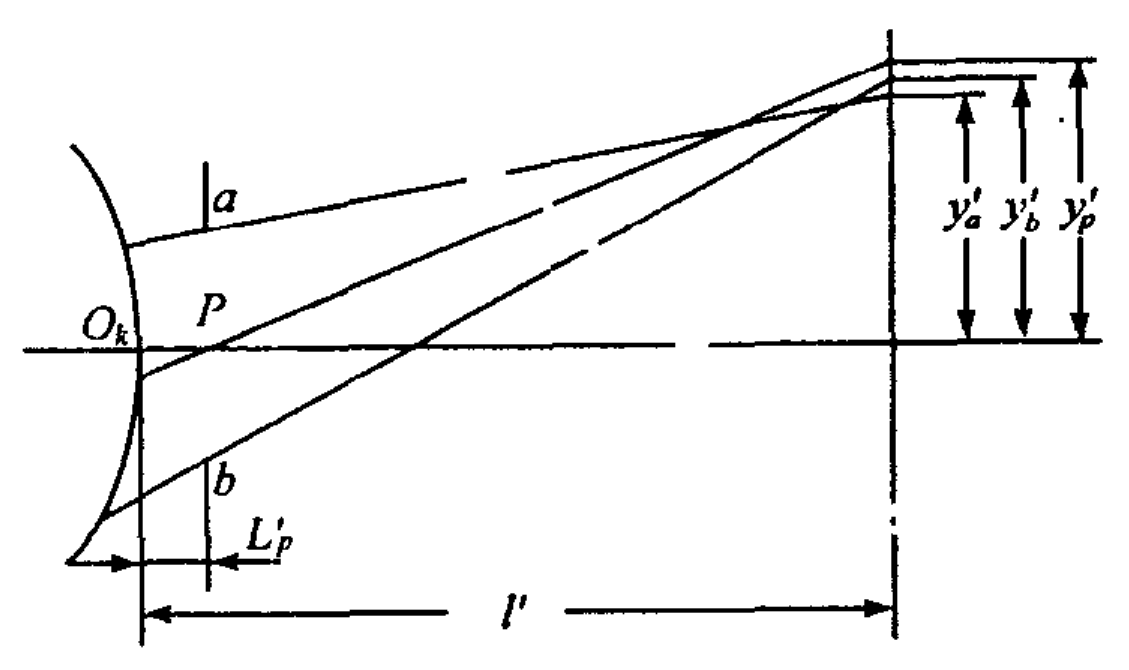
\includegraphics[width=0.6\textwidth]{coma.png}
	\caption{彗差示意图}
	\label{fig:coma}
\end{figure}

\underline{彗差是轴外点成像是产生的一种宽光束像差,是与视场和孔径有关的}。为全面了解光学系统对彗差的校正情况,需要设置多个特征视场和特征孔径计算彗差。对于子午光束,孔径取点系数为$K_{\eta}$要正负都取;对于弧矢光束,只对单向的光线计算即可,即$K_{\eta}$只取正值。

因为当光学系统不满足等晕条件,近轴轴外点就会产生彗差,所以彗差与等晕条件存在关系。可以把近轴点的弧矢彗差归结为光学系统不满足等晕条件所导致的结果。由于视场很小时主光线与高斯像面的交点高度十分接近理想高,可以证明此时有
\begin{equation}
K'_{\eta}=y'_0\cdot\mathrm{OSC}
\end{equation}

当光学系统仅由彗差时\footnote{讨论任何一种像差现象都必须把这种像差分离出来单独讨论,即认为光学系统仅存在这一种像差。},对于由出瞳出射的某一孔径带光线,其上下光线的交点在子午平面,但不在主光线上;前后光线相当于比主光线略高的一对光线但没有上下光线那么高,它们的交点在辅轴上,但不再主光线上。这个孔径带上其他任何一对光线又相当于比前后光线孔径更大,但比上下光线孔径小的光线,它们的交点应该在前后光线的交点与上下光线的交点之间。但由于它们并不关于子午面对称,所以它们的交点不在子午面内。因此,由出瞳上各个直径方向的对应点出射的各对光线在像空间相交,把这些交点连起来后将形成一个光环,光环最上方是这个光环的交点,最下方是弧矢光线的交点,其余各点对应其他的交点。孔径越大,像空间的光环也越大,相应的交点离主光线越远,于是形成了彗星状的弥散斑,如\figref{fig:lens-coma} 所示。

\begin{figure}[htbp]
	\centering
	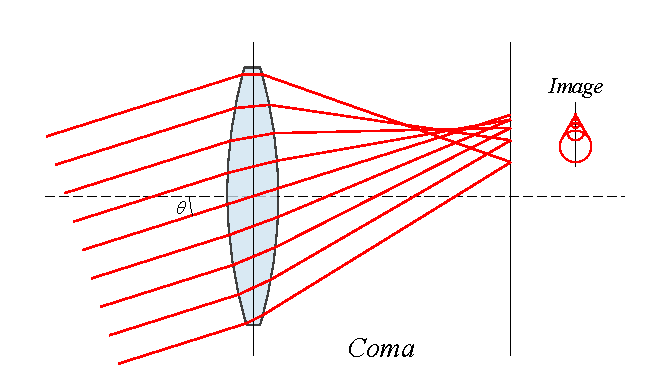
\includegraphics[width=0.6\textwidth]{lens-coma.pdf}
	\caption{彗差形成的弥散斑}
	\label{fig:lens-coma}
\end{figure}

对于单个折射球面,当主光线通过球心时满足等晕条件,不会产生彗差。这说明彗差与孔阑位置有关。因此,如果一个光学系统存在残余球差,仍可找到某一个孔阑位置使系统能够校正彗差。

\subsection{像散}
\label{subsect:astigmatism}
轴外点发出的光束,其主光线不与光学系统各个表面的对称轴重合,使出射光束失去对称。上面所述的彗差,只能表征光束失去对称的一种像差,并且是对宽光束而言的。此外,还有一种描述光束失去对称的像差。

\begin{definition}{像散}{astigmatism}
随着视场的增大,远离光轴的物点,即使在沿主光线周围的细光束范围内,也会明显地表现出失对称性质。与此细光束对应的波面也非旋转对称,而是在不同方向上有不同的曲率。数学上可以证明,一个微小的非轴对称曲面元,其曲率是随方向的变化而渐变的,但存在两条曲率分别为最大和最小的相互垂直的主截线。在光学系统中,这两条主截线正好与子午方向和弧矢方向相对应。这样,使得子午细光束和弧矢细光束,虽然因很细而能各自会聚于主光线上,但前者的会聚点$B'_t$(子午像点$T_1$)和后者的会聚点$B'_s$(弧矢像点$S_1$)并不重合,如\figref{fig:astigmatism} 所示。子午光束的会聚度大时,子午像点$B'_t$比弧矢像点$B'_s$更靠近系统,反之,$B'_s$更靠近系统。描述子午细光束和弧矢细光束会聚点之间位置差异的像差称为像散,以$B'_t$与$B'_s$之间的沿轴距离度量之,属于细光束像差。
\end{definition}

\begin{figure}[htbp]
	\centering
	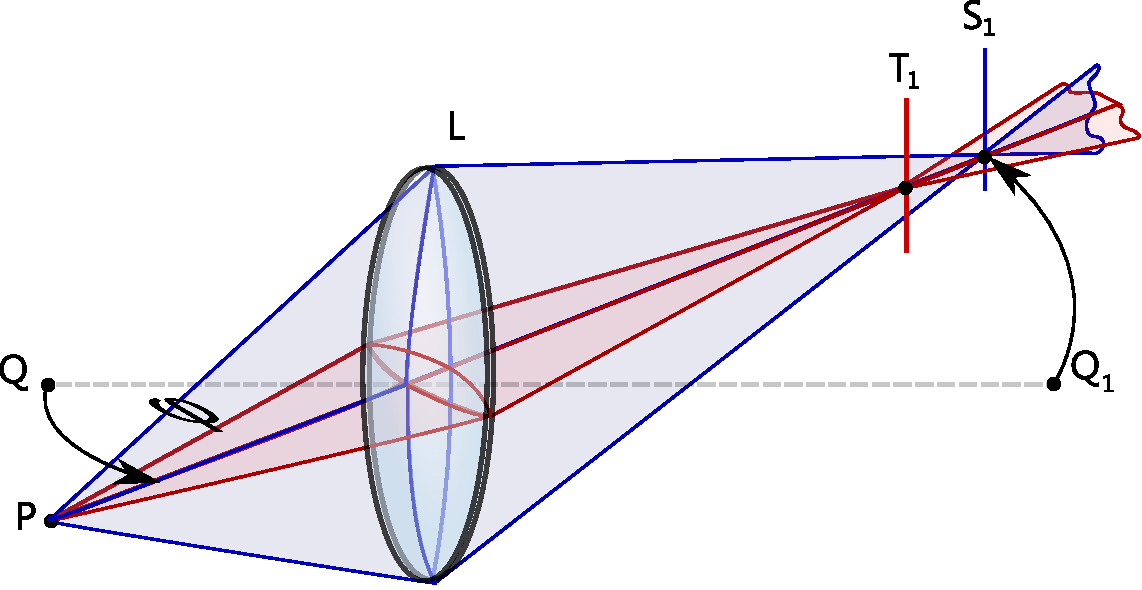
\includegraphics[width=0.6\textwidth]{astigmatism.pdf}
	\caption{像散示意图}
	\label{fig:astigmatism}
\end{figure}

\figref{fig:astigmatism} 所示为整个非对称细光束的聚焦情况。设子午光束会聚度大,即负像散。此时,在子午像点$B'_t$处聚焦成一条垂直于子午平面的短线,称为\textbf{子午焦线};在弧矢像点$B'_s$处聚焦成一条位于子午平面上的铅锤短线,称\textbf{弧矢焦线},且两个焦线互相垂直。在两条短线之间,光束的截面表现为子午焦线$\rightarrow$长轴与子午面垂直的椭圆$\rightarrow$圆$\rightarrow$长轴在子午面上的椭圆$\rightarrow$弧矢焦线。上述这种能在两个位置聚焦的非对称细光束称为像散光束。

\subsection{场曲}
\label{subsect:field-curvature}
\begin{definition}{场曲}{field-curvature}
	子午像点$B'_t$和弧矢像点$B'_s$的位置及像散的大小是随视场而异的,由这些点构成的子午像面和弧矢像面成为两个同时相切于高斯像面中心点的曲面,这就是像面弯曲,简称场曲。场曲以子午像点和弧矢像点相对于高斯像面的轴向偏离$x'_t$和$x'_s$来度量,$x'_t$称为子午场曲,$x'_t$称为弧矢场曲。二者之差,以$\Delta x$表示,即$\Delta x=x'_t-x'_s$就是同一视场的像散。
\end{definition}

为表征光学系统的像散和像面弯曲的校正情况,通常以物方视场角为纵坐标,以场曲为横坐标作曲线。为此,须对多个视场计算出场曲值。必须指出,场曲不仅仅是有像散引起的,即使像散为零,像面仍然可以是弯曲的。这就是由于第 \ref{chap:spherical-system} 章所讲的球面成像固有性质所致,这种特性被所谓匹兹凡和所决定,下文会进行讨论。为得到平的像面,必须对光学系统同时矫正像散和匹兹凡和。

无论是宽光束还是细光束,都存在子午光线的交点和弧矢光线的交点之间有沿轴距离的现象,并且这两个交点通常不在高斯像面上。所以宽光束和细光束都存在像散和场曲。实际上细光束像散和场曲是后文要讲的初级像散和场曲,一般不特别指出,像散和场曲都是指细光束的。

\subsection{畸变}
\label{subsect:distortion}
\begin{definition}{畸变}{distortion}
	对于理想光学系统,一对共轭平面上的放大率是常数。但对于实际光学系统,只当视场较小时具有这一性质,而当视场较大或很大时,像的放大率随视场而异,这样就会使像相对于物体失去相似性。这种使像形变的缺陷称为畸变。
\end{definition}

设某一视场的实际主光线与高斯像面的交点高度为$y'_p$,当无彗差时,主光线即为成像光束的中心光线,因而$y'_p$表征实际像高。它与理想像高$y'_0$之差称为\textbf{线畸变},即
\begin{equation}
\delta y'=y'_p-y'_0
\end{equation}
常用$\delta y'$相对于理想像高的百分比来表示畸变,称相对畸变,即
\begin{equation}
\frac{\delta y'}{y'_0}=\frac{y'_p-y'_0}{y'_0}\times100\%
\end{equation}
如果将实际放大率$y'_p/y$记为$\overline{\beta}$,上式可化为
\begin{equation}
\frac{\delta y'}{y'_0}=\frac{\overline{\beta}-\beta}{\beta}\times100\%
\end{equation}
式中$\beta$为理想放大率。可见,实际放大率$\overline{\beta}$与理想放大率$\beta$之差与$\beta$之比即为该视场的相对畸变。

有畸变或畸变很大的光学系统,若对等间距的同心圆物面成像,将得到非等间距的同心圆。由正畸变的光学系统所成的像呈枕型,如 \figref{fig:barrel-distortion} 所示。由负畸变光学系统所成的像呈桶型,如 \figref{fig:pincushion-distortion} 所示。

\begin{figure}[htbp]
	\centering
	\begin{minipage}[t]{0.45\textwidth}
		\centering
		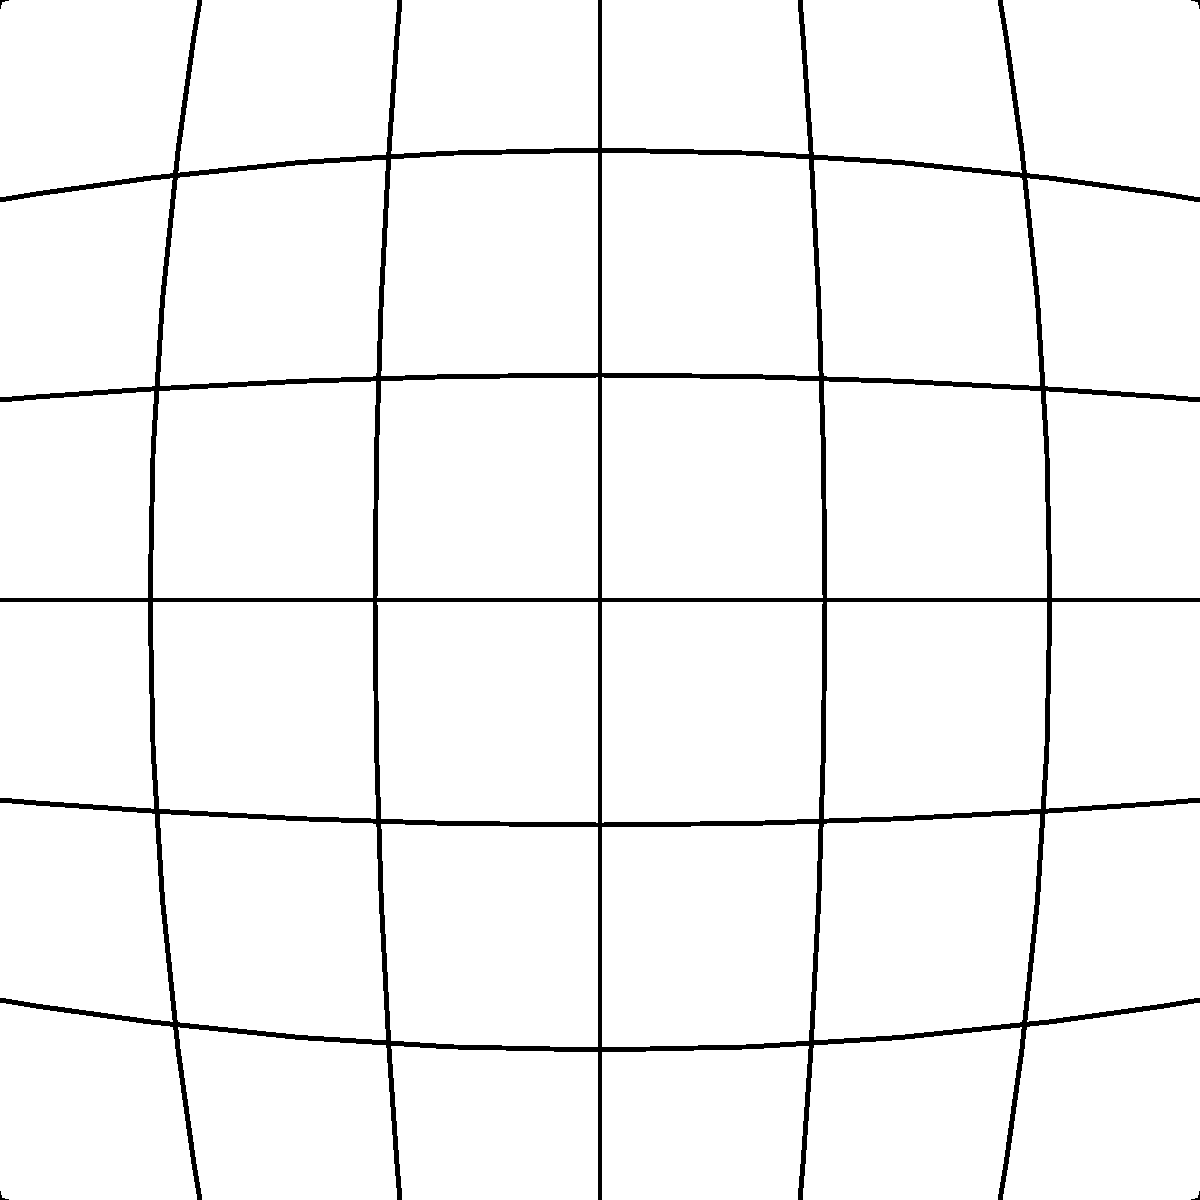
\includegraphics[width=0.6\textwidth]{barrel-distortion.pdf}
		\caption{枕形畸变}
		\label{fig:barrel-distortion}
	\end{minipage}
	\quad
	\begin{minipage}[t]{0.45\textwidth}
		\centering
		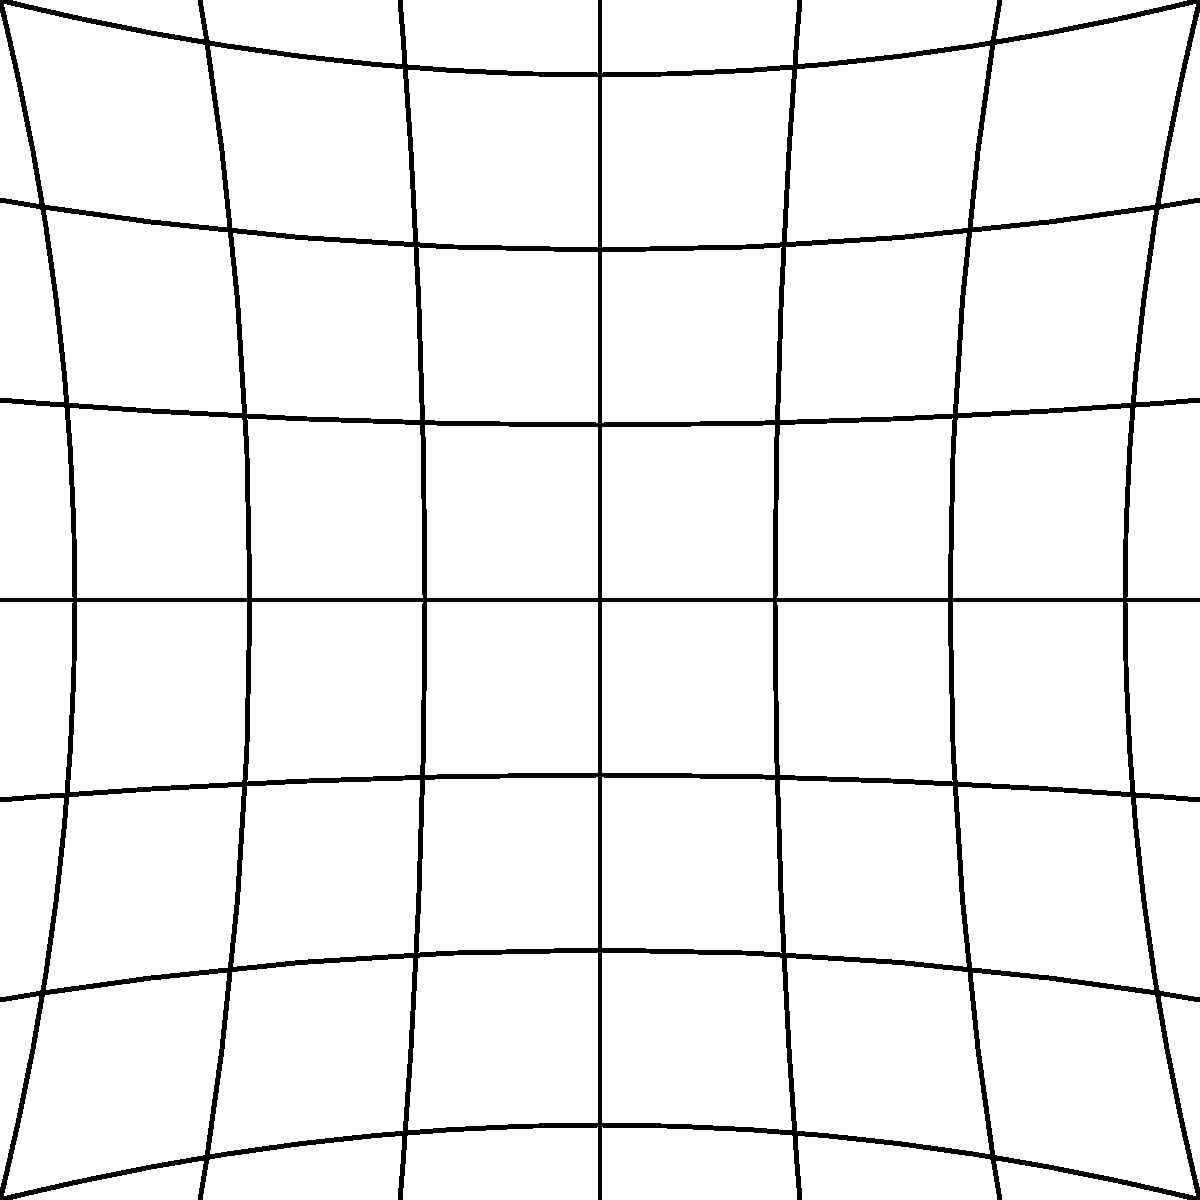
\includegraphics[width=0.6\textwidth]{pincushion-distortion.pdf}
		\caption{桶形畸变}
		\label{fig:pincushion-distortion}
	\end{minipage}
\end{figure}

可见,畸变仅由主光线的光路决定,它只引起像的形变,而对像的清晰度并无影响。因此,对于一般的光学系统,只要感觉不出它所成像的形变($\delta y'/y'_0\leqslant 4\%$),这种像差就无妨碍。但对于某些要利用像来测定物体的大小和轮廓的光学系统\footnote{如计量仪器中的投影物镜、工具显微镜以及航空测量用的摄影物镜等。计量仪器中的物镜,畸变要求小于万分之几,但视场较小,矛盾并不突出。航空测量用的物镜视场达到$120^{\circ}$,畸变要求小于十万分之几,校正相当困难,导致镜头结构极度复杂。},畸变就成为了主要的缺陷。它直接影响了测量的精度,必须严格校正。

结构完全对称的光学系统以$-1$倍的倍率成像时,畸变能自然消除。这是因为实际放大率$\overline{\beta}$可写成
\begin{equation}
\overline{\beta}=\frac{y'_p}{y}=\frac{(L'_p-l')\tan U'_p}{(L_p-l)\tan U_p}
\end{equation}
不论$U_p$为何值,由于系统的结构对称于孔径光阑,$\overline{\beta}$恒等于$-1$而不会产生畸变。

对于单个薄透镜或薄透镜组,当光阑与之重合时,主光线通过主点,沿理想方向射出,与高斯像面的交点接近,与理想像高相等,也不产生畸变。


\section{色差}
\label{sect:chromatic-aberration}
\begin{definition}{色差}{chromatic-aberration}
	当一定光谱范围内的光入射于任何形状的介质分界面时,只要入射角不为零,各种色光将因色散而有不同的传播途径,结果导致各种色光有不同的成像位置和不同的成像倍率。这种成像的色差差异称为色差。
\end{definition}

色差有两种。描述不同色光对轴上物点成像位置差异的色差称为\textbf{位置色差}或\textbf{轴向色差}。因不同色光成像倍率的不同而造成物体的像大小差异的色差称为\textbf{倍率色差}或\textbf{垂轴色差}。

\subsection{位置色差}

如\figref{fig:longitudinal-chromatic-aberration} 所示,轴上一点发出一束近轴白光,经光学系统后,$F$光交光轴于$A'_F$点,$C$光交光轴于$A'_C$。这两点是蓝光与红光所成的高斯像点。它们相对于光学系统最后一面的距离之差($l'_F-l'_C$)就是近轴光的\textbf{位置色差}$\delta l'_{ch}$,即
\begin{equation}
\delta l'_{ch}=l'_F-l'_C
\end{equation}
若两色像点重合,$l'_{ch}=0$,称光学系统对这两种色光\textbf{消色差}。通常所谓的消色差系统,即指对两种选定的色光消位置色差的系统,如\figref{fig:achromatism} 所示。

\begin{figure}[htbp]
	\centering
	\begin{minipage}[t]{0.45\textwidth}
		\centering
		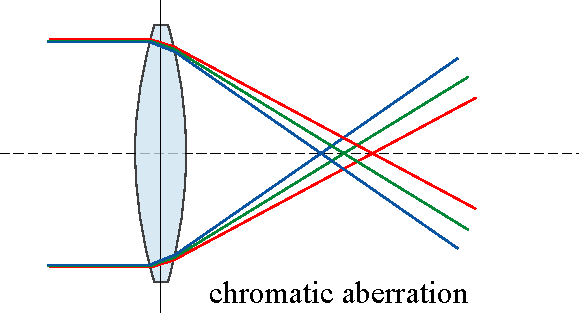
\includegraphics[width=1\textwidth]{longitudinal-chromatic-aberration.pdf}
		\caption{位置色差}
		\label{fig:longitudinal-chromatic-aberration}
	\end{minipage}
	\quad
	\begin{minipage}[t]{0.45\textwidth}
		\centering
		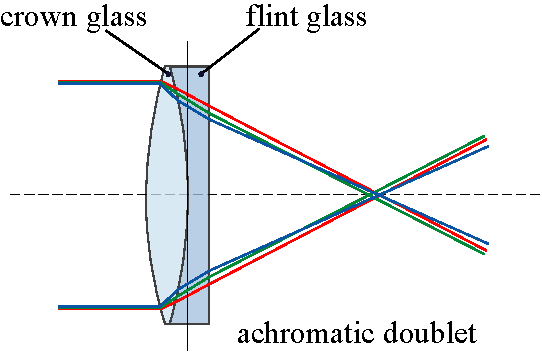
\includegraphics[width=0.95\textwidth]{achromatism.pdf}
		\caption{消色差系统}
		\label{fig:achromatism}
	\end{minipage}
\end{figure}

光学系统一般只能对光束中的某一带光线校正色差,通常是对$0.707$带光来校正。校正位置色差之后,在其他带上一定会有剩余色差。通常把计算得到的色差相对于光线的入射角$U$或入射高度$h$绘制成曲线,将上述两种色光的计算结果以球差曲线形式与主色光球差曲线画在一起,这样的曲线图不仅可以清楚地知道色差随孔径变化的情况,还可以了解到球差随色光变化的情况。这种球差的色变化称为\textbf{色球差}。

\subsection{倍率色差}
校正了位置色差的光学系统,只能使两种色光的像点或像面重合在一起,但两种色光的焦距并不一定就此相等,使这两种色光可能具有不同的放大率,使同一物体的像大小不等,因而仍可能存在\textbf{倍率色差}。

光学系统的倍率色差,用两种色光的主光线与高斯像面的交点高度之差来度量,以符号$\delta y'_{ch}$来表示,若对$F$光和$C$光考虑色差,有
\begin{equation}
\delta y'_{ch}=y'_F-y'_C
\end{equation}

倍率色差的存在,使物体像的边缘呈现颜色,影响像的清晰度。所以,具有一定大小视场的光学系统必须校正倍率色差。